\documentclass[tikz]{standalone}
\usetikzlibrary{patterns}
\usetikzlibrary{arrows}
\usetikzlibrary{decorations.shapes,decorations.markings,decorations.pathreplacing}

\tikzset{
    set arrow inside/.code={\pgfqkeys{/tikz/arrow inside}{#1}},
    set arrow inside={end/.initial=>, opt/.initial=},
    /pgf/decoration/Mark/.style={
        mark/.expanded=at position #1 with
        {
            \noexpand\arrow[\pgfkeysvalueof{/tikz/arrow inside/opt}]{\pgfkeysvalueof{/tikz/arrow inside/end}}
        }
    },
    arrow inside/.style 2 args={
        set arrow inside={#1},
        postaction={
            decorate,decoration={
                markings,Mark/.list={#2}
            }
        }
    },
}
\begin{document}
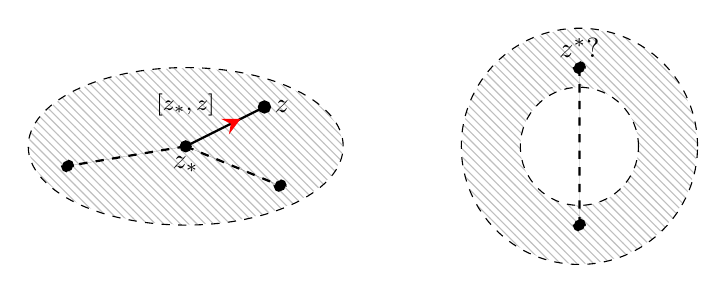
\begin{tikzpicture}
\draw[pattern=north west lines,pattern color=gray!50,draw=white] (0,0) ellipse(2 and 1);
\draw[dashed] (0,0) ellipse (2 and 1);
\draw[fill] (0,0) circle (2pt) node[below]{$z_*$};
\draw[pattern=north west lines,pattern color=gray!50,draw=white] (5,0) circle (1.5);
\draw[dashed] (5,0) circle (1.5);
\draw[dashed,fill=white] (5,0) circle (0.75);
\draw[fill,thick] (0,0) -- node[midway,above left,font=\footnotesize] {$[z_*,z]$} (1,0.5) circle (2pt) node[right]{$z$} [arrow inside={end=stealth,opt={red,scale=1.5}}{0.5}];
\draw[thick,fill,dashed] (0,0) -- (-1.5,-0.25) circle (2pt) ;
\draw[thick,fill,dashed] (0,0) -- (1.2,-0.5) circle (2pt) ;
\draw[thick,fill,dashed] (5,1)  node[above]{$z^*$?} circle (2pt) -- (5,-1) circle (2pt) ;
\end{tikzpicture}
\end{document}